% This LaTeX was auto-generated from MATLAB code.
% To make changes, update the MATLAB code and export to LaTeX again.

\documentclass{article}

\usepackage[utf8]{inputenc}
\usepackage[T1]{fontenc}
\usepackage{lmodern}
\usepackage{graphicx}
\usepackage{color}
\usepackage{hyperref}
\usepackage{amsmath}
\usepackage{amsfonts}
\usepackage{epstopdf}
\usepackage[table]{xcolor}
\usepackage{matlab}

\sloppy
\epstopdfsetup{outdir=./}
\graphicspath{ {./topt_p4_antonio_fernandez_andres_herencia_images/} }

\matlabhastoc

\begin{document}

\label{T_B44F81CE}
\matlabtitle{\textbf{PRACTICE 4 - SUPPORT VECTOR MACHINE}}

\begin{par}
\begin{flushleft}
\textbf{Andrés Herencia and Antonio Fernández}
\end{flushleft}
\end{par}

\begin{par}
\begin{flushleft}
\textbf{MUTECI 2023-2024}
\end{flushleft}
\end{par}

\matlabtableofcontents{Table of Contents}

\label{H_52219030}
\matlabheading{Exercise 1}

\begin{par}
\begin{flushleft}
From the data given in the file \texttt{svm\_nolineal.txt}, the following is requested:
\end{flushleft}
\end{par}

\begin{itemize}
\setlength{\itemsep}{-1ex}
   \item{\begin{flushleft} a) Apply the SVM model to separate lineally data into two categories. \end{flushleft}}
   \item{\begin{flushleft} b) Apply the soft model with different values of the parameter \texttt{C \textgreater{} 0} to solve the classification problem. \end{flushleft}}
   \item{\begin{flushleft} c) Use a polynomial kernel to solve the binary classification problem. If this is not possible, use the soft approach with the polynomial kernel by varying the parameter \texttt{C}. \end{flushleft}}
\end{itemize}

\begin{par}
\begin{flushleft}
\textit{\textbf{NOTE}}\textit{: use quadratic programming software and, if applicable, the appropriate kernel function.}
\end{flushleft}
\end{par}


\label{H_3380D719}
\begin{par}
\begin{flushleft}
Firstly, we will represent our data.
\end{flushleft}
\end{par}

\begin{matlabcode}
clc, clear, clf
cd 'C:\Users\andre\Documents\UNIVERSIDAD\MUTECI\BLOQUE 2\TOPT\lab\P4'
% cd 'C:\Users\anton\OneDrive\TOPT\Práctica 4'

data = importdata('svm_nolineal.txt', '\t');
X1 = data.data(:, 1); X2 = data.data(:, 2); Y = data.data(:,3);

figure(1)
gscatter(X1, X2, Y)
xlabel("x_1")
ylabel("x_2")
grid on
legend('group 1', 'group 2')
title('Original data')
\end{matlabcode}
\begin{center}
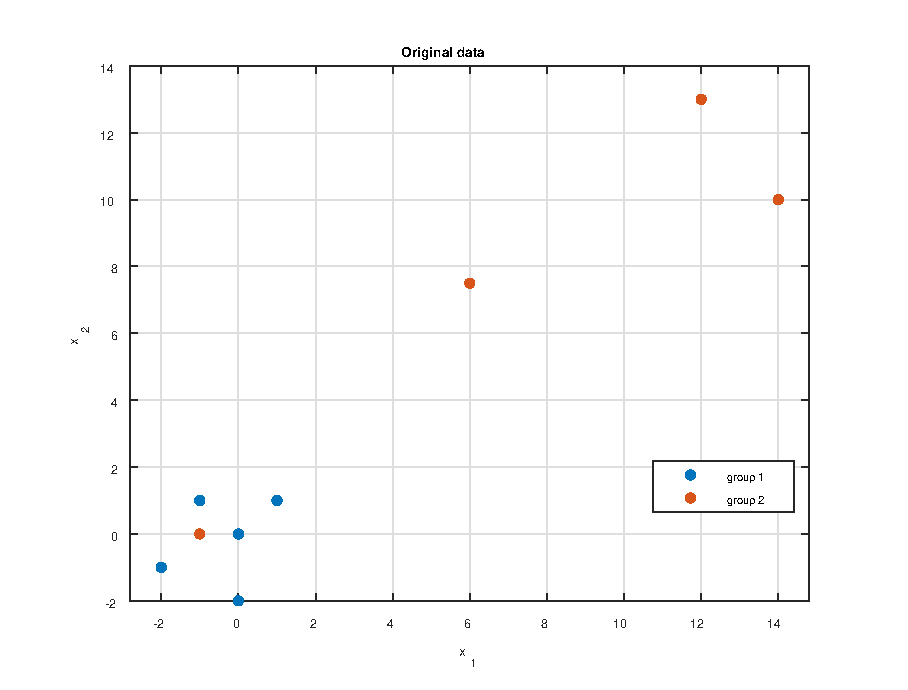
\includegraphics[width=\maxwidth{56.196688409433015em}]{figure_0.eps}
\end{center}


\label{H_28892D99}
\matlabheadingtwo{a) Apply the SVM model to separate lineally data into two categories.}

\begin{par}
\begin{flushleft}
The primal support vector machine problem will be:
\end{flushleft}
\end{par}

\begin{par}
$$P:\left\lbrace \begin{array}{cc}
{\min_{w,b} \;} & \frac{1}{2}\|w\|\\
\textrm{such}\;\textrm{to}\;\; & -y^i (w^t x^i -b)\le -1,~~\forall i\in \lbrace 1,2,\ldots,m\rbrace 
\end{array}\right.$$
\end{par}

\begin{matlabcode}
svm=fitcsvm([X1,X2],Y);
svm.Beta
\end{matlabcode}
\begin{matlaboutput}
ans = 2x1    
    0.0003
    0.3075

\end{matlaboutput}
\begin{matlabcode}
b = svm.Bias
\end{matlabcode}
\begin{matlaboutput}
b = -1.3076
\end{matlaboutput}
\begin{matlabcode}
d = 0.02;
[x1Grid,x2Grid] = meshgrid(0:d:10,0:d:10);
    
xGrid = [x1Grid(:),x2Grid(:)];
[~,scores] = predict(svm,xGrid);

figure;
h(1:2) = gscatter(X1,X2,Y,'rb','.');
hold on
X=[X1,X2];
h(3) = plot(X(svm.IsSupportVector,1),X(svm.IsSupportVector,2),'ko', 'MarkerSize',2);
contour(x1Grid,x2Grid,reshape(scores(:,2),size(x1Grid)),[0 0],'k', 'LineWidth',2);
legend(h,{'-1','+1','Support Vectors'});
grid on
xlabel("x_1")
ylabel("x_2")
hold off
\end{matlabcode}
\begin{center}
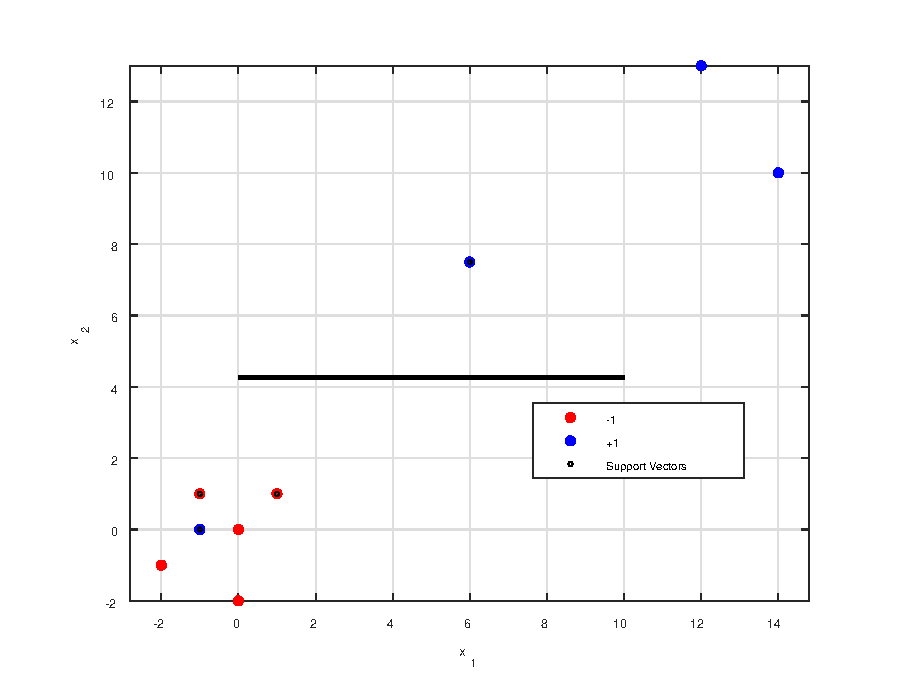
\includegraphics[width=\maxwidth{56.196688409433015em}]{figure_1.eps}
\end{center}

\begin{par}
\begin{flushleft}
How could we predict just by looking at the data, we cannot separate the two categories linearly. We will see that the quadratic problem is not feasible.
\end{flushleft}
\end{par}

\begin{matlabcode}
n = 2;
m = size(X1, 1);
H=zeros(n+1);
%indpos=Y>0;
%indneg=Y<0;
H(1:n,1:n)= eye(n);
f=zeros(n+1,1);
A=zeros(m,n+1);
A(:,1)=-1*Y.* X1;
A(:,2)=-1*Y.* X2;
A(:,3)=Y;
b= -1*ones(m,1);

quadprog(H,f,A,b,[],[],[],[]);
\end{matlabcode}
\begin{matlaboutput}
No feasible solution found.

quadprog stopped because it was unable to find a point that satisfies
the constraints within the value of the constraint tolerance.

<stopping criteria details>
\end{matlaboutput}


\label{H_A1B817F0}
\matlabheadingtwo{b) Apply the soft model with different values of the parameter \texttt{C \textgreater{} 0} to solve the classification problem.}

\begin{par}
\begin{flushleft}
\textit{\textbf{NOTE:}}\textit{ In this section, we will make use of a pre-built function, }\texttt{fitcsvm}\textit{. The soft model primal-dual problem is solved using quadratic programming in }\hyperref[H_1093E501]{\textit{Exercise 2}}\textit{.}
\end{flushleft}
\end{par}

\begin{par}
\begin{flushleft}
The soft model has the following form:
\end{flushleft}
\end{par}

\begin{par}
$$P:\left\lbrace \begin{array}{ccc}
{\min_{w,b} \;} & \frac{1}{2}+\|w\|+C\left({\sum_{i=1}^m \xi_i }\right) & \\
\textrm{such}\;\textrm{to}\;\; & y^i (w^t x^i -b)\ge 1-\xi_i ,~~ & \forall i\in \lbrace 1,2,\ldots,m\rbrace \\
 & \xi_i \ge 0,~~ & \forall i\in \lbrace 1,2,\ldots,m\rbrace 
\end{array}\right.$$
\end{par}

\begin{par}
\begin{flushleft}
The dual problem is:
\end{flushleft}
\end{par}

\begin{par}
$$D_C :\left\lbrace \begin{array}{cc}
{\min_{a\in \Re^m } \;} & \Bigl\lbrace \frac{1}{2}\sum_{j=1}^m \sum_{i=1}^m \alpha_i \alpha_i y^i y^j (x^j )^t x^i -{\left.\sum_{i=1}^m \alpha_i \Big\rbrace }\right.\\
\textrm{such}\;\textrm{to}\; & {\sum_{i=1}^m \alpha_i y^i =0~~\forall i\in \lbrace 1,2,\ldots,m\rbrace }\\
 & 0\le \alpha_i \le C,~~\forall i\in \lbrace 1,2,\ldots,m\rbrace 
\end{array}\right.$$
\end{par}

\begin{par}
\begin{flushleft}
We will try different $C$ values :\texttt{ [0.01, 1]}. We built a function that plot the decission boundary, which can be found on \hyperref[H_8B77EE59]{annexes}. 
\end{flushleft}
\end{par}

\begin{matlabcode}
C_values = [0.001, 1]; % Adjust this list as needed

% Initialize a cell array to store the SVM models
models = cell(length(C_values), 1);

% Train SVM models with different values of C
for i = 1:length(C_values)
    C = C_values(i);
    SVMModel = fitcsvm(X, Y, 'KernelFunction', 'linear', 'BoxConstraint', C);
    models{i} = SVMModel;
end


cols = 2;
rows = round(length(C_values)/cols);

% Plot the data and decision boundaries for each model
figure('Position', [100, 100, 1200, 600]);

for i = 1:length(C_values)
    subplot(rows, cols, i); % Adjust subplot parameters based on the number of C values
    SVMModel = models{i};
    h = plotDecisionBoundary(X, Y, SVMModel);
    title(['C = ' num2str(C_values(i))]);
    legend('Location', 'Best');
end
\end{matlabcode}
\begin{center}
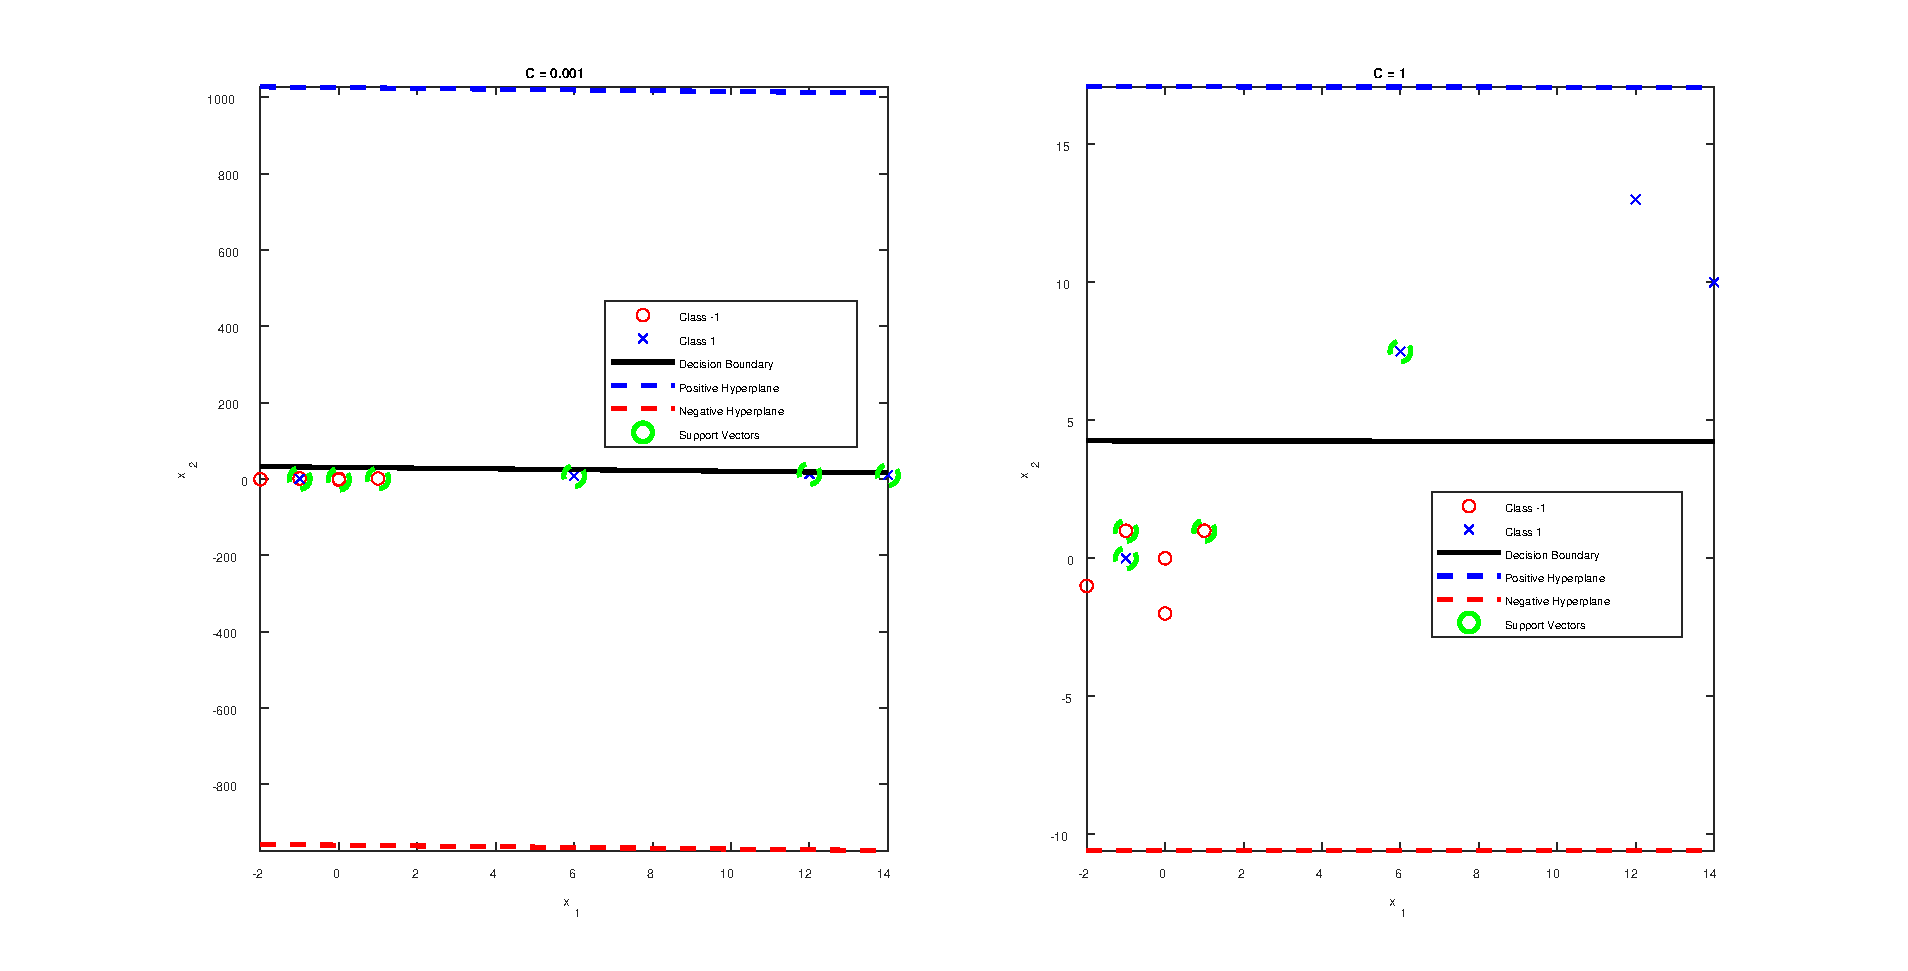
\includegraphics[width=\maxwidth{120.42147516307075em}]{figure_2.eps}
\end{center}

\begin{par}
\begin{flushleft}
We can observe how the separation line changes its slope. For $C$ values greater than 1, there are no differences in position or slope. Additionally, it can be observed that from $C=0.001$ onwards, the accuracy does not improve.
\end{flushleft}
\end{par}


\label{H_BCE9D22B}
\matlabheadingtwo{c) Use a polynomial kernel to solve the binary classification problem. If this is not possible, use the soft approach with the polynomial kernel by varying the parameter \texttt{C}.}

\begin{par}
\begin{flushleft}
Firstly, we will try to solve the problem with $C=\infty$.
\end{flushleft}
\end{par}

\begin{matlabcode}
svm=fitcsvm(X,Y,'KernelFunction','polynomial');

sv = svm.SupportVectors; 
var_dual = zeros(m,1);
var_dual(svm.IsSupportVector)=svm.Alpha;

[x1Grid,x2Grid] = meshgrid(linspace(min(X(:, 1)), max(X(:, 1)), 1000), ...
                          linspace(min(X(:, 2)), max(X(:, 2)), 1000));
    
xGrid = [x1Grid(:),x2Grid(:)];
[~,scores] = predict(svm,xGrid);

figure;
h(1:2) = gscatter(X(:,1),X(:,2),Y,'rb','.');
hold on

h(3) = plot(X(svm.IsSupportVector,1),X(svm.IsSupportVector,2),'ko');
contour(x1Grid,x2Grid,reshape(scores(:,2),size(x1Grid)),[0 0],'k');
legend(h,{'-1','+1','Support Vectors'});
axis equal
hold off
\end{matlabcode}
\begin{center}
\includegraphics[width=\maxwidth{56.196688409433015em}]{figure_3.eps}
\end{center}

\begin{par}
\begin{flushleft}
It can be observed that the polynomial kernel perfectly solves the problem, and therefore, a relaxed approach is not necessary. Anyway, let's see that with $C=1$, the result doesn't change.
\end{flushleft}
\end{par}

\begin{matlabcode}
svm = fitcsvm(X,Y,'KernelFunction','polynomial','BoxConstraint', 1);
    
[~,scores] = predict(svm,xGrid);

figure;
h(1:2) = gscatter(X(:,1),X(:,2),Y,'rb','.');
hold on

h(3) = plot(X(svm.IsSupportVector,1),X(svm.IsSupportVector,2),'ko');
contour(x1Grid,x2Grid,reshape(scores(:,2),size(x1Grid)),[0 0],'k');
legend(h,{'-1','+1','Support Vectors'});
axis equal
hold off
\end{matlabcode}
\begin{center}
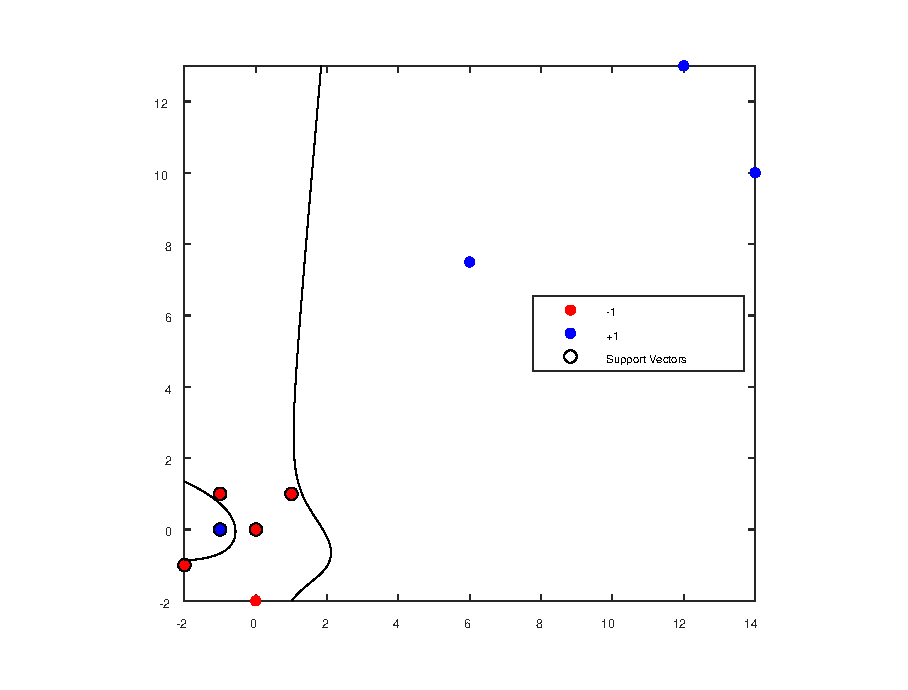
\includegraphics[width=\maxwidth{56.196688409433015em}]{figure_4.eps}
\end{center}


\label{H_1093E501}
\matlabheading{Exercise 2}

\begin{par}
\begin{flushleft}
From the data given in the file square4.txt or square4.xlsx, the following is requested:
\end{flushleft}
\end{par}

\begin{itemize}
\setlength{\itemsep}{-1ex}
   \item{\begin{flushleft} a) Apply a Support Vector Machine for separating lineally the groups 0 and 2. \end{flushleft}}
   \item{\begin{flushleft} b) Apply the soft model with different values for the parameter \texttt{C\textgreater{}0} to solve the classification problem. \end{flushleft}}
   \item{\begin{flushleft} c) Determine which value of \texttt{C} is the most suited for this problem. Justify the answer. \end{flushleft}}
\end{itemize}

\begin{matlabcode}
clear; clc; clf

data = readmatrix('square4.txt');
X1 = data(:, 1); X2 = data(:, 2); Y = data(:, 3);

figure(1)
gscatter(X1, X2, Y, 'bgrm')
grid on
xlabel("x_1")
ylabel("x_2")
legend('group 0', 'group 1','group 2', 'group 3')
title('Original data')
\end{matlabcode}
\begin{center}
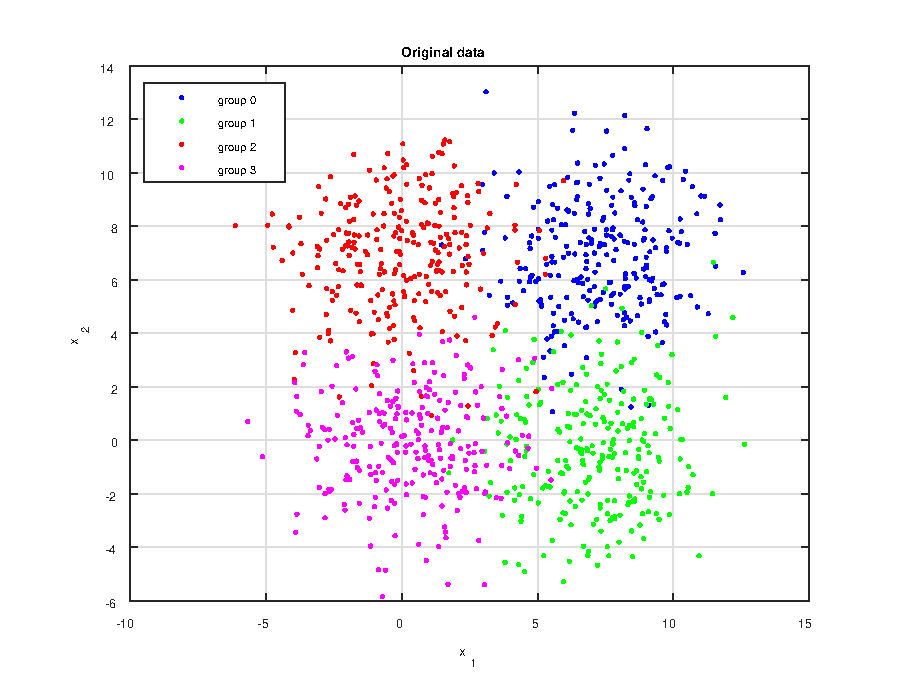
\includegraphics[width=\maxwidth{56.196688409433015em}]{figure_5.eps}
\end{center}


\label{H_5BE16A75}
\matlabheadingtwo{a) Apply a Support Vector Machine for separating lineally the groups 0 and 2.}

\begin{matlabcode}
ind1 = Y==0; 
ind2 = Y==2;
x1 = X1(ind1 | ind2);
x2 = X2(ind1 | ind2);
y = Y(ind1 | ind2);
y(y==0) = -1; y(y==2) = +1;
figure(2)
gscatter(x1, x2, y, 'br')
grid on
xlabel("x_1")
ylabel("x_2")
legend('group 0', 'group 2')
title('Group 0 and Group 2 original points')
\end{matlabcode}
\begin{center}
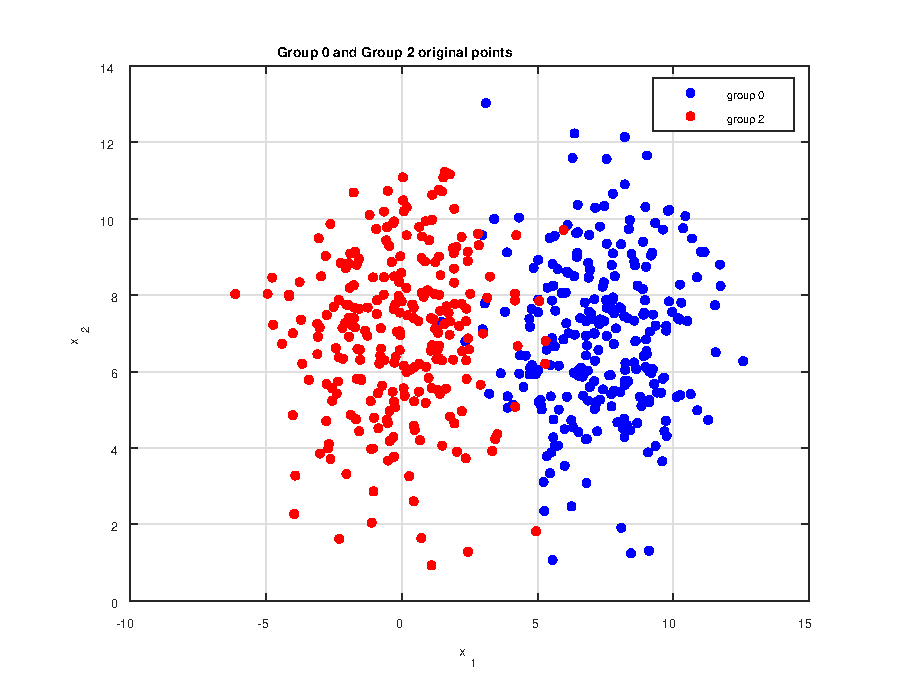
\includegraphics[width=\maxwidth{56.196688409433015em}]{figure_6.eps}
\end{center}

\begin{par}
\begin{flushleft}
We can observe graphically that there is \textbf{no linear separator for this data groups}. If we try to optimize the primal problem for the SVM...
\end{flushleft}
\end{par}

\begin{matlabcode}
% 1. Quadratic term of the objective function
n = 2; % number of groups
m = size(x1,1); % size of each group
H = zeros(n+1); % hessian
H(1:n,1:n) = eye(n)
\end{matlabcode}
\begin{matlaboutput}
H = 3x3    
     1     0     0
     0     1     0
     0     0     0

\end{matlaboutput}
\begin{matlabcode}
% 2. Linear term of the objective function (0)
f = zeros(n+1,1);
% 3. A matrix with linear conditions
A = zeros(m,n+1);
A(:,1) = -1*y.* x1; 
A(:,2) = -1*y.* x2; 
A(:,3) = y;
A
\end{matlabcode}
\begin{matlaboutput}
A = 500x3    
    6.2853   11.5879   -1.0000
    9.3978    5.4489   -1.0000
    5.7362    8.6803   -1.0000
    6.1020    9.8327   -1.0000
    9.2948    5.6737   -1.0000
    8.0270    7.6795   -1.0000
    5.0270    6.0370   -1.0000
    3.0486    7.7805   -1.0000
    2.9635    9.5684   -1.0000
    6.8647    8.8412   -1.0000

\end{matlaboutput}
\begin{matlabcode}
% b term
b = -1*ones(m,1);
[wb,ff,exitflag] = quadprog(H,f,A,b,[],[],[],[])
\end{matlabcode}
\begin{matlaboutput}
No feasible solution found.

quadprog stopped because it was unable to find a point that satisfies
the constraints within the value of the constraint tolerance.

<stopping criteria details>
wb = 3x1    
   -0.2891
    0.0096
   -0.9591

ff = 0.0418
exitflag = -2
\end{matlaboutput}

\begin{par}
\begin{flushleft}
We can see that, indeed, there is no feasible solution to this problem.
\end{flushleft}
\end{par}

\begin{par}
\begin{flushleft}
A lot of points have been misclassified. Then, we need to "relax" this model for penalizing those points that would have been misclassified using a soft model. 
\end{flushleft}
\end{par}


\label{H_093C362E}
\matlabheadingtwo{b) Apply the soft model with different values for the parameter \texttt{C\textgreater{}0} to solve the classification problem.}

\begin{par}
\begin{flushleft}
The soft model has the following form:
\end{flushleft}
\end{par}

\begin{par}
$$P:\left\lbrace \begin{array}{ccc}
{\min_{w,b} \;} & \frac{1}{2}+\|w\|+C\left({\sum_{i=1}^m \xi_i }\right) & \\
\textrm{such}\;\textrm{to}\;\; & y^i (w^t x^i -b)\ge 1-\xi_i ,~~ & \forall i\in \lbrace 1,2,\ldots,m\rbrace \\
 & \xi_i \ge 0,~~ & \forall i\in \lbrace 1,2,\ldots,m\rbrace 
\end{array}\right.$$
\end{par}

\begin{par}
\begin{flushleft}
From the previous model, they have been included $m$ variables $\xi_i \ge 0$ to identify those points $x^i$ that have been misclassified. These variables act on those points that are on the wrong side of the plane and penalize them based on their value.
\end{flushleft}
\end{par}

\begin{par}
\begin{flushleft}
On the other hand, the value of $C$ penalizes failure to comply with prior constraints. This is, the higher the value, the greater the penalization. In the limit case, when $C\to \infty$ tends to be infinite, the previous model converges to the first model with the proposed separator hyperplane ($H$), narrowing the band where the hyperplane $H^+$ and $H^-$ are located. Meanwhile, a low value ($C\to 0$) will widen the strip, allowing it to contain more points that should be misclassified.
\end{flushleft}
\end{par}

\begin{par}
\begin{flushleft}
The dual problem is:
\end{flushleft}
\end{par}

\begin{par}
$$D_C :\left\lbrace \begin{array}{cc}
{\min_{a\in \Re^m } \;} & \Bigl\lbrace \frac{1}{2}\sum_{j=1}^m \sum_{i=1}^m \alpha_i \alpha_i y^i y^j (x^j )^t x^i -{\left.\sum_{i=1}^m \alpha_i \Big\rbrace }\right.\\
\textrm{such}\;\textrm{to}\; & {\sum_{i=1}^m \alpha_i y^i =0~~\forall i\in \lbrace 1,2,\ldots,m\rbrace }\\
 & 0\le \alpha_i \le C,~~\forall i\in \lbrace 1,2,\ldots,m\rbrace 
\end{array}\right.$$
\end{par}

\begin{par}
\begin{flushleft}
We can determine the vector ${\bar{w} }$ in the same way as the strict model does, as a function of $\bar{\alpha}$: ${\bar{w} }=\sum_{i=1}^m \bar{\alpha_i } y^i x^i$.
\end{flushleft}
\end{par}

\begin{par}
\begin{flushleft}
Thus, to solve this problem we have to:
\end{flushleft}
\end{par}

\begin{itemize}
\setlength{\itemsep}{-1ex}
   \item{\begin{flushleft} 1.- Characterize the quadratic term of the objective function. \end{flushleft}}
   \item{\begin{flushleft} 2.- Compute the linear term of the objective function. \end{flushleft}}
   \item{\begin{flushleft} 3.- Obtain the equation matrix and the independent term of the objective function. \end{flushleft}}
   \item{\begin{flushleft} 4.- Apply the model with some values of $C$ and represent graphically their hyperplane bounds. We will take the following values of C in a logarithmic scale, between \texttt{1e-4} and \texttt{1e+4.} \end{flushleft}}
   \item{\begin{flushleft} 5.- Compare the models (in section c). \end{flushleft}}
\end{itemize}

\begin{matlabcode}
% 1.
H=(([x1,x2]).*y)*([x1,x2].*y)'
\end{matlabcode}
\begin{matlaboutput}
H = 500x500    
  173.7845  122.2091  136.6408  152.2927  124.1673  139.4411  101.5518  109.3217  129.5043  145.5974  157.7962   93.9872  114.5039  137.9891  117.5149  158.3637  117.1311  143.4792  102.8121  108.3664  110.6915   92.1133  159.3635  182.2620   60.2119  115.6694  123.8295   96.6178  144.7858  119.7137  108.9778  117.3941  175.5962  132.7111  144.5838  132.7649  138.3224  165.2499   83.2250  125.7261   89.6637   91.8553  131.5489  162.1242  131.4256   93.3501   91.3886  136.3067   84.6107  113.8252
  122.2091  118.0082  101.2060  110.9220  118.2657  117.2806   80.1371   71.0455   79.9874  112.6873  132.1376   84.3864  110.6684  104.0266  101.0641  128.9394  108.0038  124.9511   94.0900   95.5426   99.7840   85.2082  121.9488  152.9783   62.1041  117.0141  111.2479   91.7710  109.5993   95.8587   92.0616  113.8740  158.0378  117.7996  130.7156  105.7924  105.9462  131.5513   76.1692  131.7686   80.7407   66.6422  119.9602  150.5331   93.0251   58.9598   76.0032  112.6638   75.6966  105.2930
  136.6408  101.2060  108.2526  120.3531  102.5670  112.7051   81.2387   85.0253  100.0563  116.1218  127.4482   76.8179   94.8411  109.6115   95.3381  127.3204   96.1867  116.6510   84.3148   88.2904   90.5345   75.6859  126.8788  147.2650   50.4960   96.6393  101.2194   79.7694  115.0820   95.9895   88.1471   97.3008  143.5793  108.2516  118.3154  106.3718  110.1425  132.3788   68.2524  105.7724   73.3219   72.5494  107.8130  133.3009  103.4318   72.3311   73.7286  109.8557   69.1110   93.5258
  152.2927  110.9220  120.3531  133.9152  112.5044  124.4901   90.0338   95.1060  112.1661  128.8204  140.8079   84.5465  103.9404  121.7581  105.1804  140.8760  105.7043  128.6052   92.6974   97.2721   99.6206   83.1597  140.8341  162.6818   55.1235  105.6211  111.3993   87.5122  127.8088  106.3016   97.3413  106.6132  158.0034  119.2190  130.1684  117.8290  122.2512  146.6444   75.0378  115.3509   80.6855   80.7399  118.5560  146.4325  115.2443   81.0077   81.4871  121.4555   76.0795  102.7612
  124.1673  118.2657  102.5670  112.5044  118.5843  118.1807   80.9768   72.4809   81.8336  113.9682  133.1765   84.8068  110.9061  105.3374  101.7450  130.1103  108.4287  125.7280   94.4878   96.0885  100.2652   85.5328  123.3995  154.1660   62.0926  117.0721  111.7994   92.0278  110.9590   96.8001   92.7510  114.1034  158.8101  118.4405  131.3309  106.8545  107.2019  132.8776   76.4910  131.6717   81.1335   67.6058  120.4841  151.0848   94.4849   60.2451   76.6232  113.6128   76.0846  105.6941
  139.4411  117.2806  112.7051  124.4901  118.1807  123.4072   86.7123   84.2216   97.2681  122.9984  139.3034   86.3785  109.9464  114.9094  105.3360  137.6025  109.3497  129.5430   95.5560   98.5421  101.9700   86.1574  133.7929  161.1137   60.1585  114.1941  113.8453   91.8068  120.8383  103.0532   96.6884  112.9687  161.6078  121.1552  133.4191  113.9782  116.1870  141.7907   77.3541  126.8684   82.5465   74.9302  122.0077  151.9785  105.8151   70.8944   80.3637  119.4460   77.5985  106.4657
  101.5518   80.1371   81.2387   90.0338   80.9768   86.7123   61.7154   62.2961   72.6615   87.8824   97.9684   59.8981   75.1119   82.5360   73.6826   97.3215   75.4196   90.3861   66.0065   68.5848   70.6525   59.3851   95.8128  113.2542   40.5610   77.2963   78.9350   62.9409   86.7234   73.1308   67.8781   77.1199  112.0106   84.2082   92.3884   80.9630   83.1892  100.7386   53.4326   85.2629   57.2069   54.2331   84.3392  104.6738   76.9634   52.7307   56.5962   84.2244   53.8487   73.3828
  109.3217   71.0455   85.0253   95.1060   72.4809   84.2216   62.2961   69.8310   83.4821   89.7170   95.4137   55.7973   66.5479   85.5329   70.5737   96.4249   69.0211   85.8833   60.7127   64.6529   65.6415   54.2294   98.4530  110.1431   34.2833   66.2760   73.5015   56.4456   89.6643   73.1847   65.7487   68.1526  104.1773   79.0329   85.6711   81.2573   85.4361  101.1624   49.1452   71.2053   53.1877   57.4106   77.7603   95.3444   82.5654   59.9391   55.3549   82.6887   50.2801   67.0117
  129.5043   79.9874  100.0563  112.1661   81.8336   97.2681   72.6615   83.4821  100.3369  104.9395  110.2727   63.7173   74.9095  100.4139   81.2044  111.9389   78.4267   98.6078   69.0848   74.0718   74.9036   61.5815  115.3429  127.2481   38.0402   73.8682   83.9251   63.7648  105.2047   85.1763   75.8790   76.6578  118.9121   90.4379   97.7071   94.6408  100.0798  117.8413   55.9216   78.7075   60.7047   67.7430   88.5428  108.1923   97.7298   71.8752   64.0465   95.7662   57.4543   76.0966
  145.5974  112.6873  116.1218  128.8204  113.9682  122.9984   87.8824   89.7170  104.9395  125.2903  139.0025   84.6183  105.6147  117.8528  104.3724  138.3225  106.3665  127.9331   93.1352   97.0007   99.7858   83.7355  136.6890  160.6678   56.7931  108.3661  111.5074   88.5999  123.8018  104.0460   96.2568  108.4129  158.2139  119.0468  130.4606  115.2231  118.6733  143.3753   75.3932  119.2592   80.8016   77.6144  119.0296  147.5594  110.3028   76.0616   80.3355  119.5975   76.0893  103.4728

\end{matlaboutput}
\begin{matlabcode}
% 2. 
f=-1*ones(m,1)
\end{matlabcode}
\begin{matlaboutput}
f = 500x1    
    -1
    -1
    -1
    -1
    -1
    -1
    -1
    -1
    -1
    -1

\end{matlaboutput}
\begin{matlabcode}
% 3.
Aeq = zeros(1,m);
Aeq(1,:) = y'
\end{matlabcode}
\begin{matlaboutput}
Aeq = 1x500    
    -1    -1    -1    -1    -1    -1    -1    -1    -1    -1    -1    -1    -1    -1    -1    -1    -1    -1    -1    -1    -1    -1    -1    -1    -1    -1    -1    -1    -1    -1    -1    -1    -1    -1    -1    -1    -1    -1    -1    -1    -1    -1    -1    -1    -1    -1    -1    -1    -1    -1

\end{matlaboutput}
\begin{matlabcode}
beq = 0
\end{matlabcode}
\begin{matlaboutput}
beq = 0
\end{matlaboutput}


\label{H_5547AEAE}
\matlabheadingthree{Parameter C = 10\textasciicircum{}-4}

\begin{par}
\hfill \break
\end{par}

\begin{matlabcode}
C0 = 1e-4;
[pr0, ph0] = svm_soft(x1,x2,y,H,f,Aeq,beq,C0,true)
\end{matlabcode}
\begin{matlaboutput}
Minimum found that satisfies the constraints.

Optimization completed because the objective function is non-decreasing in 
feasible directions, to within the value of the optimality tolerance,
and constraints are satisfied to within the value of the constraint tolerance.

<stopping criteria details>
\end{matlaboutput}
\begin{center}
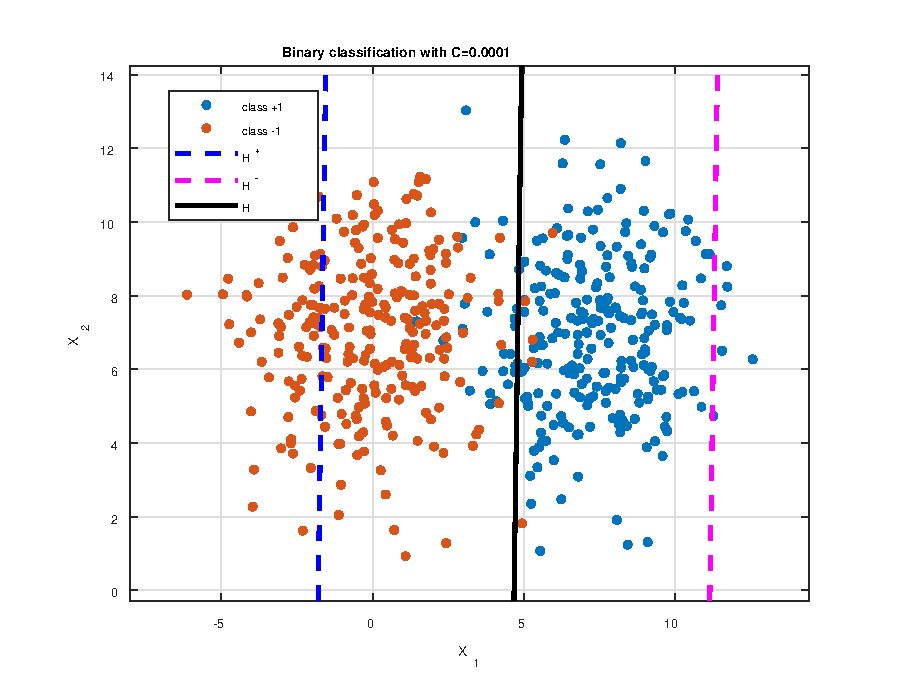
\includegraphics[width=\maxwidth{56.196688409433015em}]{figure_7.eps}
\end{center}
\begin{matlaboutput}
pr0 = 0.9420
ph0 = 0.1360
\end{matlaboutput}


\label{H_F6C0AA3F}
\matlabheadingthree{Parameter C = 10\textasciicircum{}-3}

\begin{par}
\hfill \break
\end{par}

\begin{matlabcode}
C1 = 0.001
\end{matlabcode}
\begin{matlaboutput}
C1 = 1.0000e-03
\end{matlaboutput}
\begin{matlabcode}
[pr1, ph1] = svm_soft(x1,x2,y,H,f,Aeq,beq,C1,true)
\end{matlabcode}
\begin{matlaboutput}
Minimum found that satisfies the constraints.

Optimization completed because the objective function is non-decreasing in 
feasible directions, to within the value of the optimality tolerance,
and constraints are satisfied to within the value of the constraint tolerance.

<stopping criteria details>
\end{matlaboutput}
\begin{center}
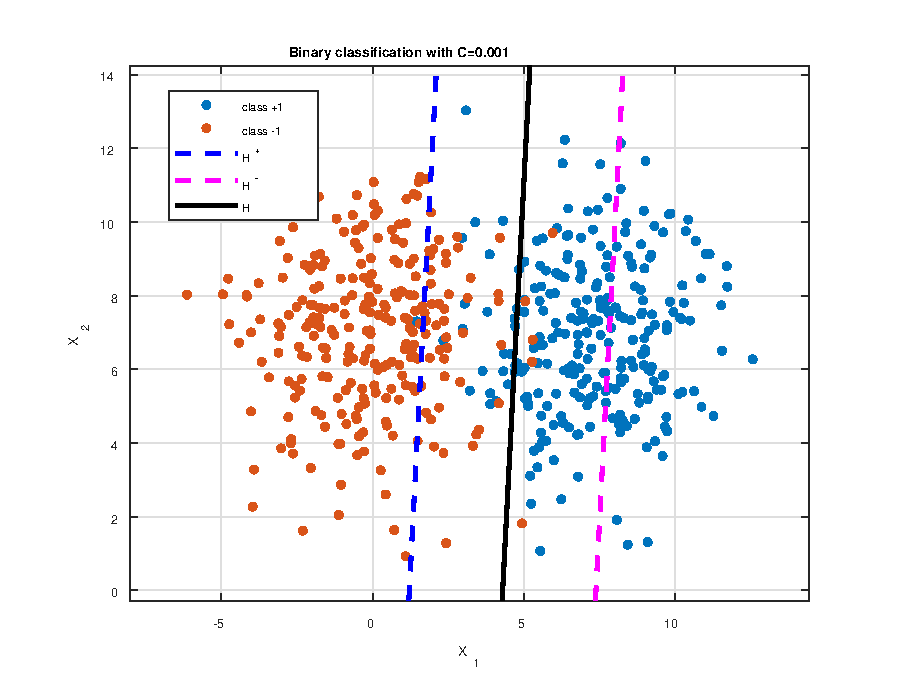
\includegraphics[width=\maxwidth{56.196688409433015em}]{figure_8.eps}
\end{center}
\begin{matlaboutput}
pr1 = 0.9440
ph1 = 0.6040
\end{matlaboutput}


\label{H_83972684}
\matlabheadingthree{Parameter C = 0.01}

\begin{par}
\hfill \break
\end{par}

\begin{matlabcode}
C2 = 1e-2;
[pr2, ph2] = svm_soft(x1,x2,y,H,f,Aeq,beq,C2,true)
\end{matlabcode}
\begin{matlaboutput}
Minimum found that satisfies the constraints.

Optimization completed because the objective function is non-decreasing in 
feasible directions, to within the value of the optimality tolerance,
and constraints are satisfied to within the value of the constraint tolerance.

<stopping criteria details>
\end{matlaboutput}
\begin{center}
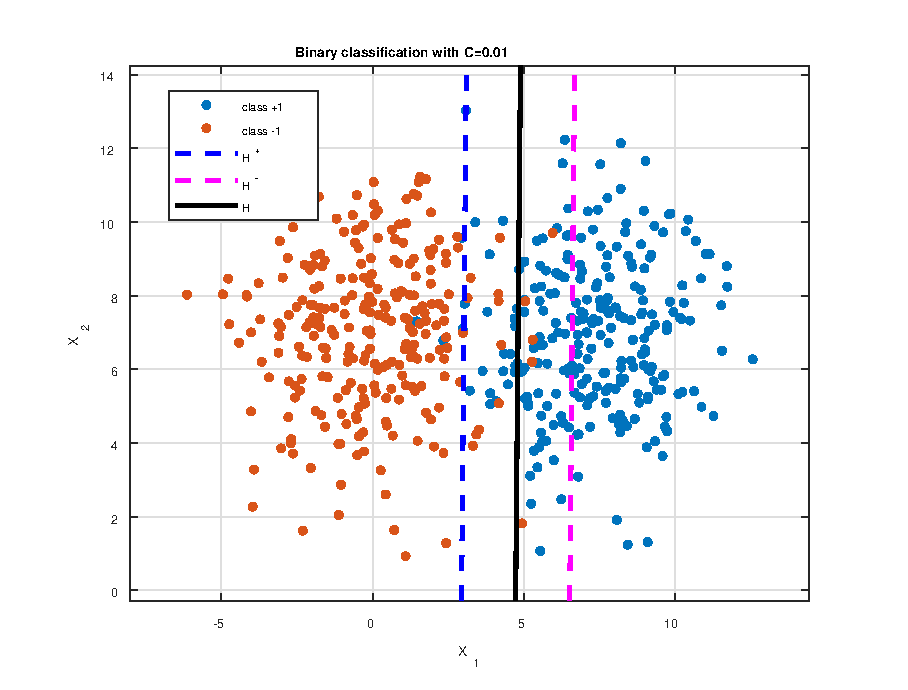
\includegraphics[width=\maxwidth{56.196688409433015em}]{figure_9.eps}
\end{center}
\begin{matlaboutput}
pr2 = 0.9400
ph2 = 0.7980
\end{matlaboutput}


\label{H_EAD42ADD}
\matlabheadingthree{Parameter C = 0.1}

\begin{par}
\hfill \break
\end{par}

\begin{matlabcode}
C3 = 1e-1;
[pr3, ph3] = svm_soft(x1,x2,y,H,f,Aeq,beq,C3,true)
\end{matlabcode}
\begin{matlaboutput}
Minimum found that satisfies the constraints.

Optimization completed because the objective function is non-decreasing in 
feasible directions, to within the value of the optimality tolerance,
and constraints are satisfied to within the value of the constraint tolerance.

<stopping criteria details>
\end{matlaboutput}
\begin{center}
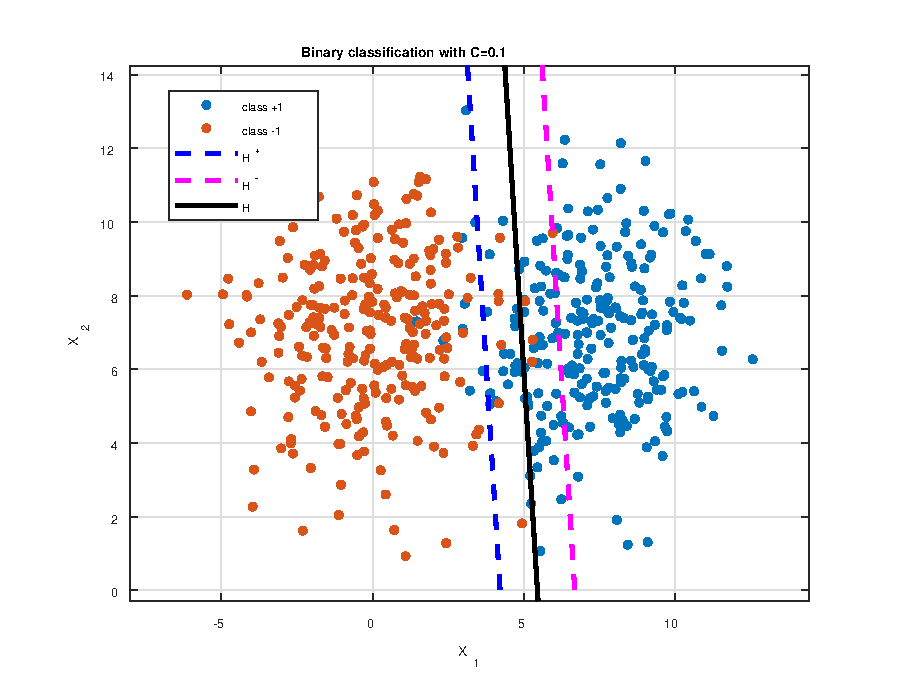
\includegraphics[width=\maxwidth{56.196688409433015em}]{figure_10.eps}
\end{center}
\begin{matlaboutput}
pr3 = 0.9340
ph3 = 0.8560
\end{matlaboutput}


\label{H_B6FA3E31}
\matlabheadingthree{Parameter C = 1}

\begin{par}
\hfill \break
\end{par}

\begin{matlabcode}
C4 = 1;
[pr4, ph4] = svm_soft(x1,x2,y,H,f,Aeq,beq,C4,true)
\end{matlabcode}
\begin{matlaboutput}
Minimum found that satisfies the constraints.

Optimization completed because the objective function is non-decreasing in 
feasible directions, to within the value of the optimality tolerance,
and constraints are satisfied to within the value of the constraint tolerance.

<stopping criteria details>
\end{matlaboutput}
\begin{center}
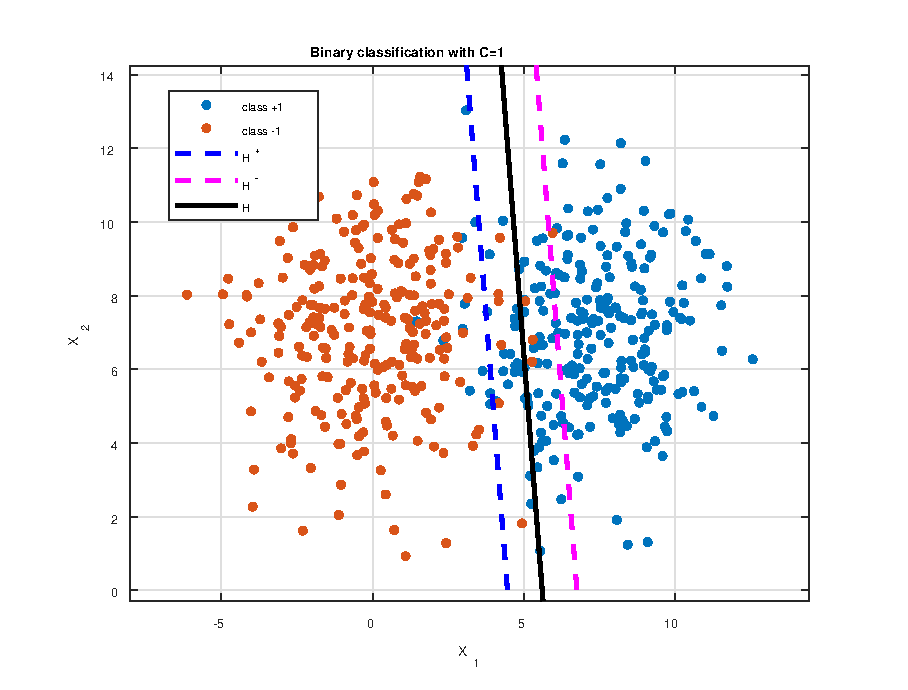
\includegraphics[width=\maxwidth{56.196688409433015em}]{figure_11.eps}
\end{center}
\begin{matlaboutput}
pr4 = 0.9300
ph4 = 0.8640
\end{matlaboutput}

\begin{par}
\begin{flushleft}
From now on forward, the quadratic optimization problem associated with computing the optimum hyperplane distance returns the same result. Then, we will not show those plots.
\end{flushleft}
\end{par}


\label{H_435854D0}
\matlabheadingthree{Parameter C = 10}

\begin{par}
\hfill \break
\end{par}

\begin{matlabcode}
C5 = 1e1;
[pr5, ph5] = svm_soft(x1,x2,y,H,f,Aeq,beq,C5,false);
\end{matlabcode}
\begin{matlaboutput}
Minimum found that satisfies the constraints.

Optimization completed because the objective function is non-decreasing in 
feasible directions, to within the value of the optimality tolerance,
and constraints are satisfied to within the value of the constraint tolerance.

<stopping criteria details>
\end{matlaboutput}


\label{H_34DD46CA}
\matlabheadingthree{Parameter C = 100}

\begin{par}
\hfill \break
\end{par}

\begin{matlabcode}
C6 = 1e2;
[pr6, ph6] = svm_soft(x1,x2,y,H,f,Aeq,beq,C6,false);
\end{matlabcode}
\begin{matlaboutput}
Minimum found that satisfies the constraints.

Optimization completed because the objective function is non-decreasing in 
feasible directions, to within the value of the optimality tolerance,
and constraints are satisfied to within the value of the constraint tolerance.

<stopping criteria details>
\end{matlaboutput}


\label{H_E70283AF}
\matlabheadingthree{Parameter C = 1000}

\begin{par}
\hfill \break
\end{par}

\begin{matlabcode}
C7 = 1e3;
[pr7, ph7] = svm_soft(x1,x2,y,H,f,Aeq,beq,C7,false);
\end{matlabcode}
\begin{matlaboutput}
Minimum found that satisfies the constraints.

Optimization completed because the objective function is non-decreasing in 
feasible directions, to within the value of the optimality tolerance,
and constraints are satisfied to within the value of the constraint tolerance.

<stopping criteria details>
\end{matlaboutput}


\label{H_8C1C4CA5}
\matlabheadingthree{Parameter C = 10\textasciicircum{}4}

\begin{par}
\hfill \break
\end{par}

\begin{matlabcode}
C8 = 1e4;
[pr8, ph8] = svm_soft(x1,x2,y,H,f,Aeq,beq,C8,true);
\end{matlabcode}
\begin{matlaboutput}
Minimum found that satisfies the constraints.

Optimization completed because the objective function is non-decreasing in 
feasible directions, to within the value of the optimality tolerance,
and constraints are satisfied to within the value of the constraint tolerance.

<stopping criteria details>
\end{matlaboutput}
\begin{center}
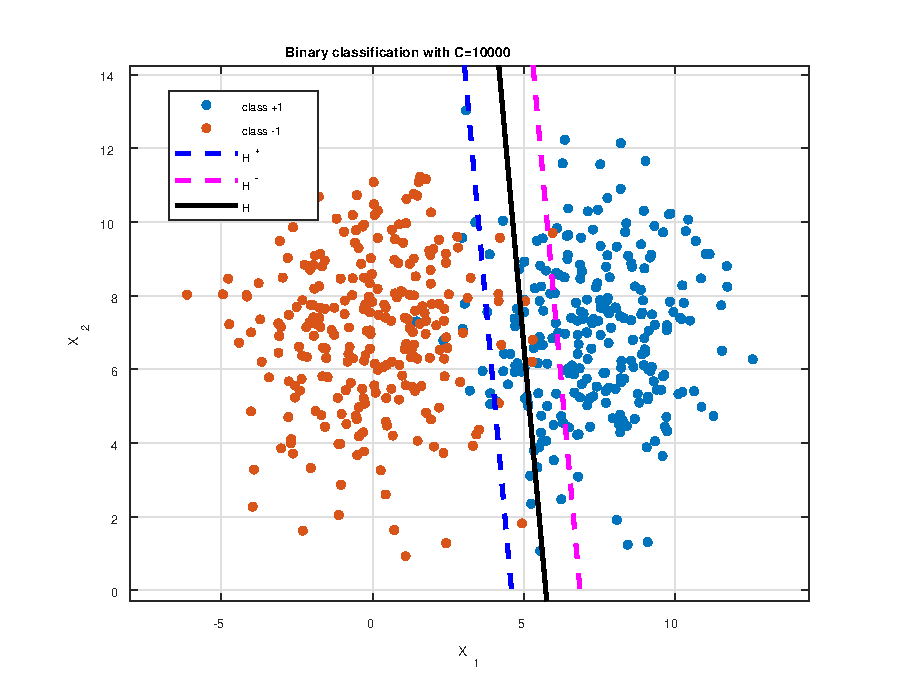
\includegraphics[width=\maxwidth{56.196688409433015em}]{figure_12.eps}
\end{center}


\label{H_9FEF4DA8}
\matlabheadingtwo{c) Determine which value of C is the most suited for this problem. Justify the answer.}

\begin{par}
\begin{flushleft}
Now we must determine which value of $C$ is the most suited for this binary classification. 
\end{flushleft}
\end{par}

\begin{matlabcode}
% Definir tus datos
pr = [pr0, pr1, pr2, pr3, pr4, pr5, pr6, pr7, pr8].*100;
C = [C0, C1, C2, C3, C4, C5, C6, C7, C8];

figure;
semilogx(C, pr, 'bo-');
ylabel('Accuracy (%)');
xlabel('C values');

grid on;
title('Performance comparison between models');

ax = gca;
chart = ax.Children(1);
datatip(chart,0.001,94.4);
\end{matlabcode}
\begin{center}
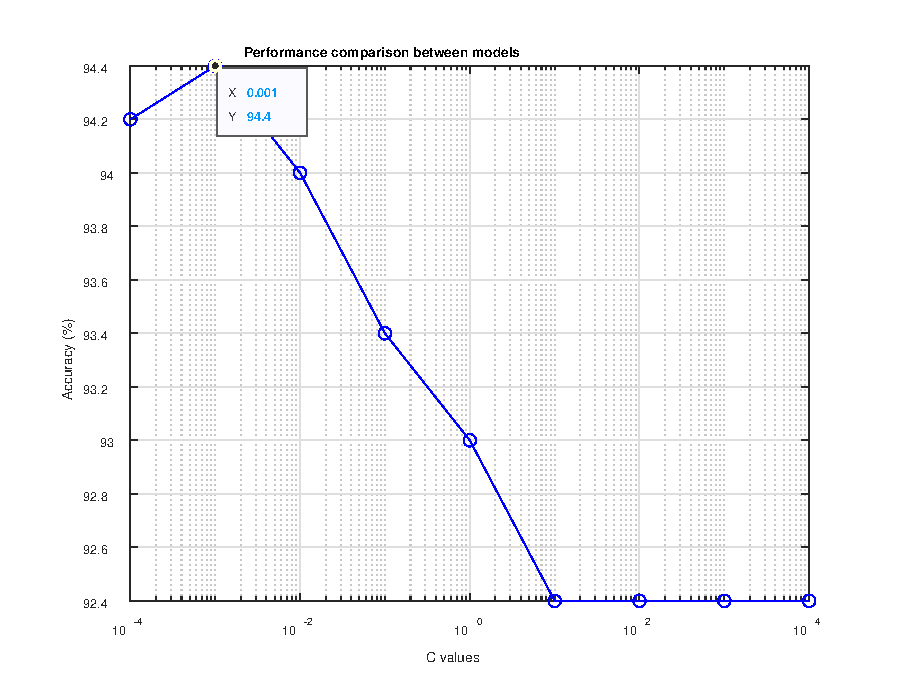
\includegraphics[width=\maxwidth{56.196688409433015em}]{figure_13.eps}
\end{center}

\begin{par}
\begin{flushleft}
As we can see, the accuracy gets better when $C=10^{-3}$. But in general, a low value of C allows us to get better results, because both groups are too mixed between them, and a wider margin penalizes less those points.
\end{flushleft}
\end{par}


\label{H_21EFC4B0}
\matlabheading{Annexes}

\label{H_E0960C96}
\matlabheadingtwo{Exercise 1}

\label{H_8B77EE59}
\matlabheadingthree{Plot decision boundary for SVM soft model}

\begin{par}
\begin{flushleft}
This function takes a SVMModel trained with the package \texttt{fitcsvm.}
\end{flushleft}
\end{par}

\begin{matlabcode}
function h = plotDecisionBoundary(X, Y, SVMModel)
%% Description:
%  Plots the decision boundary, positive hyperplane, negative hyperplane, 
%  and support vectors for the given SVM model.
%
%  Inputs:
%  - X: Input data matrix with two features.
%  - Y: Vector of class labels (-1 or 1).
%  - SVMModel: SVM model trained using fitcsvm.
%
%  Outputs:
%  - h: Figure handle.

gscatter(X(:, 1), X(:, 2), Y, 'rb', 'ox');
hold on;

% Extract parameters
k = SVMModel.KernelParameters.Scale;
b = SVMModel.Bias;

% Calculate slope and intercept
slope = -SVMModel.Beta(1) / SVMModel.Beta(2);
intercept = b / SVMModel.Beta(2);

% Plot decision boundary
xline = linspace(min(X(:, 1)), max(X(:, 1)), 100);
yline = slope * xline - intercept;
plot(xline, yline, 'k-', 'LineWidth', 2);

% Plot positive hyperplane
yline_pos = slope * xline - (intercept - 1) / SVMModel.Beta(2);
plot(xline, yline_pos, 'b--', 'LineWidth', 2);

% Plot negative hyperplane
yline_neg = slope * xline + (intercept + 1) / SVMModel.Beta(2);
plot(xline, yline_neg, 'r--', 'LineWidth', 2);

% Highlight support vectors
idx = SVMModel.IsSupportVector;
plot(X(idx, 1), X(idx, 2), 'go', 'MarkerSize', 10, 'LineWidth', 2);
hold off;
xlabel('x_1');
ylabel('x_2');
legend('Class -1', 'Class 1', 'Decision Boundary', ...
    'Positive Hyperplane', 'Negative Hyperplane', 'Support Vectors');
axis tight;
h = gcf;

end
\end{matlabcode}

\label{H_FDC95ED7}
\matlabheadingtwo{Exercise 2}

\label{H_D27C9F57}
\matlabheadingthree{SVM soft model using quadratic programming.}

\begin{par}
\hfill \break
\end{par}

\begin{matlabcode}
function [performance_rate, points_bet_hyp] = svm_soft(x1, x2, y, H, f, Aeq, beq, C, plt)
%% Description:
% Own-made MATLAB function implements a Support Vector Machine (SVM) with a 
% soft margin for binary classification.
%
% Inputs:
% - x1: Feature values for the first dimension.
% - x2: Feature values for the second dimension.
% - y: Class labels (+1 or -1).
% - H: Hessian matrix in the quadratic programming problem.
% - f: Linear coefficient vector in the quadratic programming problem.
% - Aeq: Coefficients for linear equality constraints.
% - beq: Values for linear equality constraints.
% - C: Regularization parameter for the soft margin.
% - plt: Boolean indicating whether to plot the decision boundaries and support vectors (true or false).
%
% Outputs:
% - performance_rate: The rate of correctly classified data points.
% - points_bet_hyp: The proportion of data points located between the decision boundaries.

% Lower and upper bound for the alpha value.
m= size(x1,1);
lb = zeros(m,1);
ub = C * ones(m,1);

[alpha, fun, exitflag] = quadprog(H, f, [], [], Aeq, beq, lb, ub);

if exitflag == -2
    return
else
    % normal vector to the hyperplanes
    w = [x1,x2]'*(alpha.*y);

    % identify support vectors for the class +1:
    for i=1:m
        if y(i) > 0
            indk = i;
        else
            indh = i;
        end
    end

    b = ([x1(indk),x2(indk)]*w + [x1(indh),x2(indh)]*w)/2;

    % Plotting
    % indneg = y<0; indpos = y>0;
    % H^+
    xx1 = min(x1):0.1:max(x1);
    xx2p = (b + 1 - w(1) * xx1)./ w(2);
    % H^-
    xx2n = (b - 1 - w(1) * xx1)./ w(2);
    % H
    xx2 = (b - w(1) * xx1)./ w(2);

    if plt == true
        gscatter(x1, x2, y)
        hold on
        plot(xx1,xx2p,'b--',xx1,xx2n,'m--', xx1,xx2,'k-','LineWidth',2);
        title("Binary classification with C="+num2str(C));
        xlabel('X_1');
        ylabel('X_2');
        ylim([min(x2) - abs(max(x2) - min(x2))/10, ...
            max(x2) + abs(max(x2) - min(x2))/10]);
        xlim([min(x1) - abs(max(x1) - min(x1))/10, ...
            max(x1) + abs(max(x1) - min(x1))/10]);
        legend('class +1','class -1','H^+','H^-','H')
        grid on
        hold off
    end

    % parameters of each hyperplane
    Xx1 = [ones(length(xx1),1), xx1'];
    bn = Xx1\xx2n';
    bp = Xx1\xx2p';
    bh = Xx1\xx2';
    hn = @(x1) bn(1) + bn(2).*x1;
    hp = @(x1) bp(1) + bp(2).*x1;
    h = @(x1) bh(1) + bh(2).*x1;

    % points in a wrong class
    missclassified = 0;
    % points between hyperplanes
    points_hyperplane = 0;
    % validation criterion

    % checking if wether the points fits in the hyperplane or are
    % misclassified
    for k = 1:length(x1)
        if bn(2) < 0
            if (x2(k) > hn(x1(k))) || (x2(k) < hp(x1(k)))
                points_hyperplane = points_hyperplane + 1;
            end
            if (x2(k) > h(x1(k))) && (y(k) ~= -1) || (x2(k) < h(x1(k))) && (y(k) ~= 1)
                missclassified = missclassified + 1;
            end
        else
            if (x2(k) < hn(x1(k))) || (x2(k) > hp(x1(k)))
                points_hyperplane = points_hyperplane + 1;
            end
            if (x2(k) < h(x1(k))) && (y(k) ~= -1) || (x2(k) > h(x1(k))) && (y(k) ~= 1)
                missclassified = missclassified + 1;
            end
        end
    end
    performance_rate = (length(x1)-missclassified)/length(x1);
    points_bet_hyp = points_hyperplane/length(x1);
end
end
\end{matlabcode}

\end{document}
